\subsection{Cost benefit analyse}
\label{Cost_Ben}
Da vi skulle implementere vores system var det vigtigt for os at vi valgte den korrekt implementations strategi i forhold til hvor meget benefit brugeren ville få ud af de forskellige løsninger. Vi overvejede derfor hvilken benefit brugerne ville få af at vi brugte en platform frem for en anden  og hvor meget det ville koste os at implementere det, for at få et overblik over hvordan disse ting forholdte sig til hinanden valgt vi at lave et skema der vist benefit af en implementation kontra costen.

\begin{figure}[h!]
  \centering
    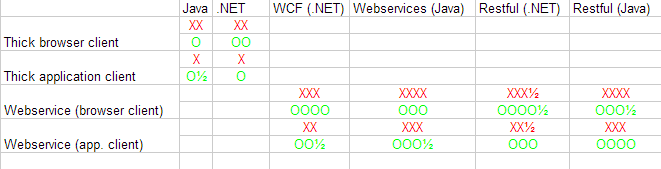
\includegraphics[width=0.5\textwidth]{Appendix/GUI-Prototype/CostBenefit}
  \caption{Tabel over cost/benefit i forhold til de forskellige implementations muligheder}
\label{Cost_Ben}
\end{figure} 

Figur \ref{Cost_Ben} viser vores cost benefit skema over de forskellige implementationsmuligheder, de røde X'er repræsenterer costen for at implementere den tilsvarende kombination. Måden hvorpå vi kom frem til hvad costen af de forskellige implementations muligheder, var at tage udgangspunkt i om vi først skulle tilegne os viden eller om vi allerede havde den fornødende forståelse til at kunne gå igang med det samme. Derefter kiggede vi på hvor meget kode der skulle skrives til de forskellige implementationsmodeller for at kunne få et fungerende system, eksempelvis er "Java, Thick browser client" dyre end "Java, Thick application client" da vi ikke vidst hvordan man lavede en browser client i java og alle Webservice løsningerne er dyre en Thick client løsningerne da der skal kodes en del mere hvis der skal laves en webservice.

De grønne O'er repræsenterer de benefits som brugeren får af den givne implementationsmodel. Måden hvorpå vi kom frem til hvad benefit af implementationsmulighederne var hvor mange platforme det understøttede eksmepelvis synes vi, at det gav brugeren mere benefit hvis deres system kunne køre på alle computer i en browser end hvis man skulle downloade en klient og tjekke om den kunne køre på computeren. Derudover kiggede vi også på hvor nemt det ville være for brugeren at udvikle videre på systemet, eksempelvis giver implementationsmuligheden "WCF(.NET), Webservice(browser client)" brugeren mulighed for at udvikle en applikation til windows phone da der er en service at kode op imod.

Udfra de måder at vudere cost og benefit vuderede vi at den løsning hvor kunden ville få mest benefit var "Restful(.NET), Webservice (browser client)" da det ville give slut brugeren mulighed for at kunne køre systemet på stort set alle computere med internet connection, og de ville være i stand til at lave en mobil applikation op imod webservicen.

 